\documentclass{article}
\usepackage{amsmath,amssymb,braket,url,hyperref,booktabs,graphicx}
\usepackage[style=nature]{biblatex}
\addbibresource{12_ref.bib}
\newcommand{\bfit}[1]{\textit{\textbf{#1}}}
\begin{document}
\medskip
\noindent
\textbf{\Large Chapter 12\\
Electron Spin Qubit in Semicoductor-1-Qubit and 2-Qubit Gates}\\\\\\
\medskip
\textbf{\large 12.1 Introduction}\\
In Chap.11, we showed how to implement a qubit using electron spin on a silicon
substrate. We also demonetrated how to initialize and measure a qubit. In this chapter,
we will sudy how to perform a universal 1-qubit gate and a 2-qubit entnaglement gate to fulfill
the last two DiVincenzo's criteria (Sect. 1.3). In Chap.10, we showed
that by applying a vertical DC magnetic field and a rotating  horizontal magnetic field and
then \textit{working in the rotating frame}, we would be able to rotate any state on Bloch sphere
about any vector. This allows us to build a universal 1-qubit gate (Section 27.4 in \cite{WongHuiYong})
However, in the literature, many silicon qubits are still implemented with the setup in Chap. 9 which means
that the qubit is places in a vertical DC magnetic field and a perturbating and linearly oscillating horizontal
magnetic field. This is what we will use in this chapter. We will first summarize an experimental paper on how
it implements 1-qubit gate. Then we will discuss the implementation of a 2-qubit entnaglement gate with an example.
\\\\\\
\bfit{\large 12.1.1 Learning Outcomes}
\\\\
Be able to describe how a 1-qubit gate can be implemented for silicon spin qubits; 
understant how a CNOT-gate can be impelmented by using a native entanglement gate of
silicon spin qubits and other 1-qubit gates.
\\\\
\bfit{\large 12.1.2 Teaching Videos}\\\\
$\bullet$ Search for Ch12 in this playlist\\

- \url{https://tinyurl.com/3yhze3jn}\\\\
$\bullet$ Other Videos\\

- \url{https://youtu.be/0JVw4xICV10}

- \url{https://youtu.be/_CpQ-Uy0Kgo}
\\\\\\
\textbf{\large 12.2 1-Qubit Gate Implementation}
\\\\
We will use an example in \cite{veldhorst2014addressable} (with some variation)
to demonstrate how to implement electron spin qubit in silicon and the 1-qubit gate.
The setup is illustrated in Fig. 12.1.

Firstly, the Hilbert space is created by applying a DC magnetic field pointing to the right.
This direction is named the $-\hat{z}$ direction. Therefore, \textit{spin-up means that the spin is 
pointing to the left, and spin-down means that the spin is pointing to the right}. This is nothing
special becuase the name of direction is completely a human definition.

The system is kept at 50 mK and $B_0=1.4T$. This is a spin qubit. To enhance the decoherence
time, we need to avoid the spin interacting with the external environment. The electron spin can
interact with the nuclear spin in the silicon easily and lose its coherence.
Unfortunately, while 95.53\% of natural silicon atoms have a zero nuclear spin
(92.23\% $^{28}Si$ \textbf{isotope} and 3.1\% $^{30}Si$ isotope), 4.67\% of them have
a spin ($^{29}Si$ isotope). This is because $^{29}Si$ has 14 protons and 15 neutrons
and their spins are not nullified due odd number of nucleons. The electron spin will interact
strongly with the nucleus of $^29Si$. Therefore, a highly purified silicon substrate is used,
in which $^29Si$ is reduced to 800 $ppm$ (part-per-million). That means, among 1 million silicon
atoms in the substrate, only 800 will be $^{29}Si$.
\\\\

      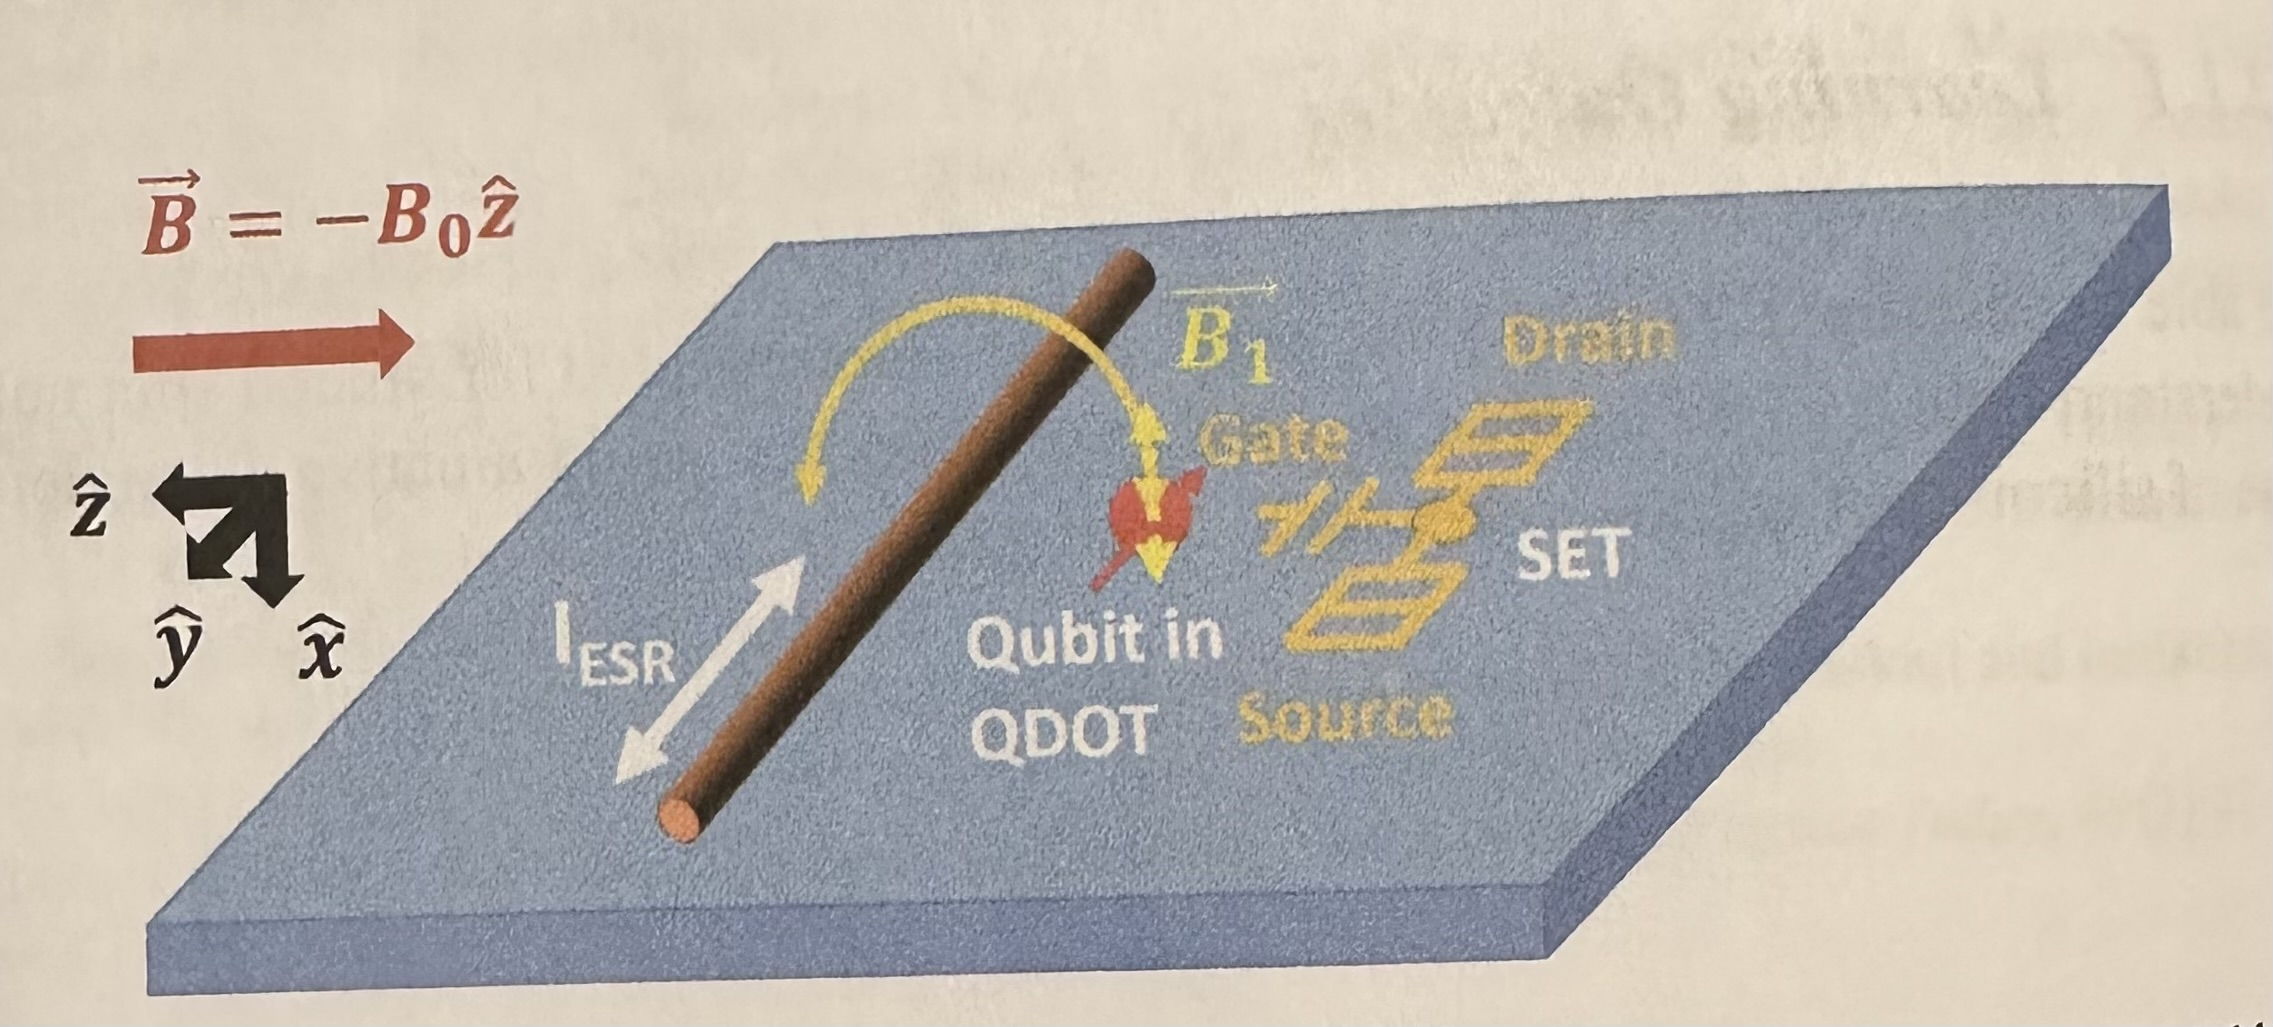
\includegraphics[scale=0.55]{Fig.12.1.jpeg}\\
\textbf{Fig. 12.1} Illustration of how an electron spin qubit is implemented in 
  \cite{veldhorst2014addressable}. The magnetic field due to $I_{ESR}$ is shown and it points
  perpendicular to the substrate at the qubit
\\\\

For \textbf{readout}, it also uses spin-to-charge conversion as in Sect. 11.6. However, instead of using a 
qunatum point contact (QPC) transistor, it uses a \textbf{single electron transistor} (SET) which has its current
also very sensitive to the charge occupation in the quantum dot.

To implement a 1-qubit gate, it uses the theory we learned in Sect 9.3. That is by applying a perturbing oscillating
magnetic field in the $\hat{x}$ direction. But note that, the $\hat{x}$ direaction in Fig.12.1 is perpendicular to the silicon substrate.
To achieve the oscillating magnetic field, an AC electric current, $I_{ESR}$, is passed through
a wire next to the qubit. $ESR$ stands for \textbf{electron spin resonance} which means that its
frequency is the same as the Larmor frequency due to $\vec{B}$ (see Sect.9.4). The current will generate a circular
magnetic field about the wire due to the \textbf{Biot-Savart law} (see
also Example 24.2). Although it is circular, at the point where it touches the qubit, it is pointing
at the tangential direction of the circle and thus it is pointing in the $\hat{x}$ direction and perpendicular
to the Si substrate. Since $I_{ESR}$ in an AC current, the magnetic field at the qubit oscillates up and down
and has the equation form given in the first term of Eq. (9.5). And as discussed in Sect. 9.6, in therotating frame,
any state will rotate about the $\hat{x^\prime}$ due to Rabi oscillation. Combined with Larmor precession, it can be used
to implement any 1-qubit gate.\\\\\\
\textbf{\large 12.3 2-Qubit Gate for Spin Inmplementation}\\\\
A 2-qubit gate is usually much more difficult to implement than a 1-qubit gate. We also need to recall that, to form
a universal set of quantum gates, what we need is not an arbitary 2-qubit gate but an \textbf{entanglement gate}, which 
can be used to create entanglements (see Sect. 4.6). Entanglement is one of the reasons that makes quantum computing superior
to classical computing.

A 2-qubit gate requires the interaction between two qubits and the external excitation under an appropriate Hamiltonian.
It is not difficult to appreciate that different quatum computer architectures have different "native" entnaglement gates because 
the physics is fairly different in different quantum computing archtectures. Here, a \textbf{native entanglement gate} is a gate that 
can be implemented easily using the physics relevant to a given architecture and its controls.

\textit{One of thenative entanglement gates} for an electron spin qubit is a special form of the controlled
phase shift gate. We will call it $\boldsymbol{U_{Cphase}}$ \cite{meunier2011efficient} to distinguish it from 
$\boldsymbol{U_{C P S, \pi}}$ in Section 16.4 in \cite{WongHuiYong},
\begin{equation}\label{eq 12.1}
  \boldsymbol{U_{Cphase}}=\begin{pmatrix}
    1&0&0&0\\0&e^{i\phi}&0&0\\0&0&e^{i(\pi-\phi)}&0\\0&0&0&1
  \end{pmatrix}.\tag{12.1}
\end{equation}
where $\phi$ is the phase. We will discuss how to implement it soon. We will first show how it can be used to create an entanglement.
\\\\\\
\bfit{\large 12.3.1 Creation of Entanglement}
\\\\
We have learned that we can use $C N O T$ gate, $\boldsymbol{U_{XOR}}$ to make two qubits entangled (Section 15.4 in \cite{WongHuiYong} and Sect.4.6). This is
realized with the help of a Hadamard gate, \bfit{H}. This circuit is shown in Fig. 12.2.

The circuit implement the following operations:
\begin{align*}\label{eq 12.2}
  \boldsymbol{U_{XOR}}(\ket{0}\otimes\ket{0})&=\boldsymbol{U_{XOR}}(\frac{1}{\sqrt{2}}(\ket{0}+\ket{1})\otimes\ket{0}).\\
  &=\boldsymbol{U_{XOR}}\frac{1}{\sqrt{2}}(\ket{00}+\ket{10}),\\
  &=\frac{1}{\sqrt{2}}(\ket{00}+\ket{11}),\tag{12.2}
\end{align*}
where we used the difinitions of $\boldsymbol{H}$ and $\boldsymbol{U_{XOR}}$ in line 1 and line 3, respectively.
We can use \textbf{controlled phase shift gate} with a phase shift of $\pi$ ($\boldsymbol{U_{CPS,\pi}}$) (see Section 16.4
in \cite{WongHuiYong}) to implement the $\boldsymbol{U_{XOR}}$ gate \textit{by combining it with other 1-qubit gates}.
\\\\
\textbf{Example 12.1} Show that $\boldsymbol{U_{XOR}}=(\boldsymbol{I}\otimes\boldsymbol{H})\boldsymbol{U_{CPS,\pi}}(\boldsymbol{I}\otimes\boldsymbol{H})$.

Firstly the matrix form of $\boldsymbol{U_{XOR}}$ is
\begin{equation}\label{eq 12.3}
  \boldsymbol{U_{XOR}}=\begin{pmatrix}
    1\ 0\ 0\ 0\\ 0\ 1\ 0\ 0\\ 0\ 0\ 0\ 1\\ 0\ 0\ 1\ 0
  \end{pmatrix}\tag{12.3}
\end{equation}
\\

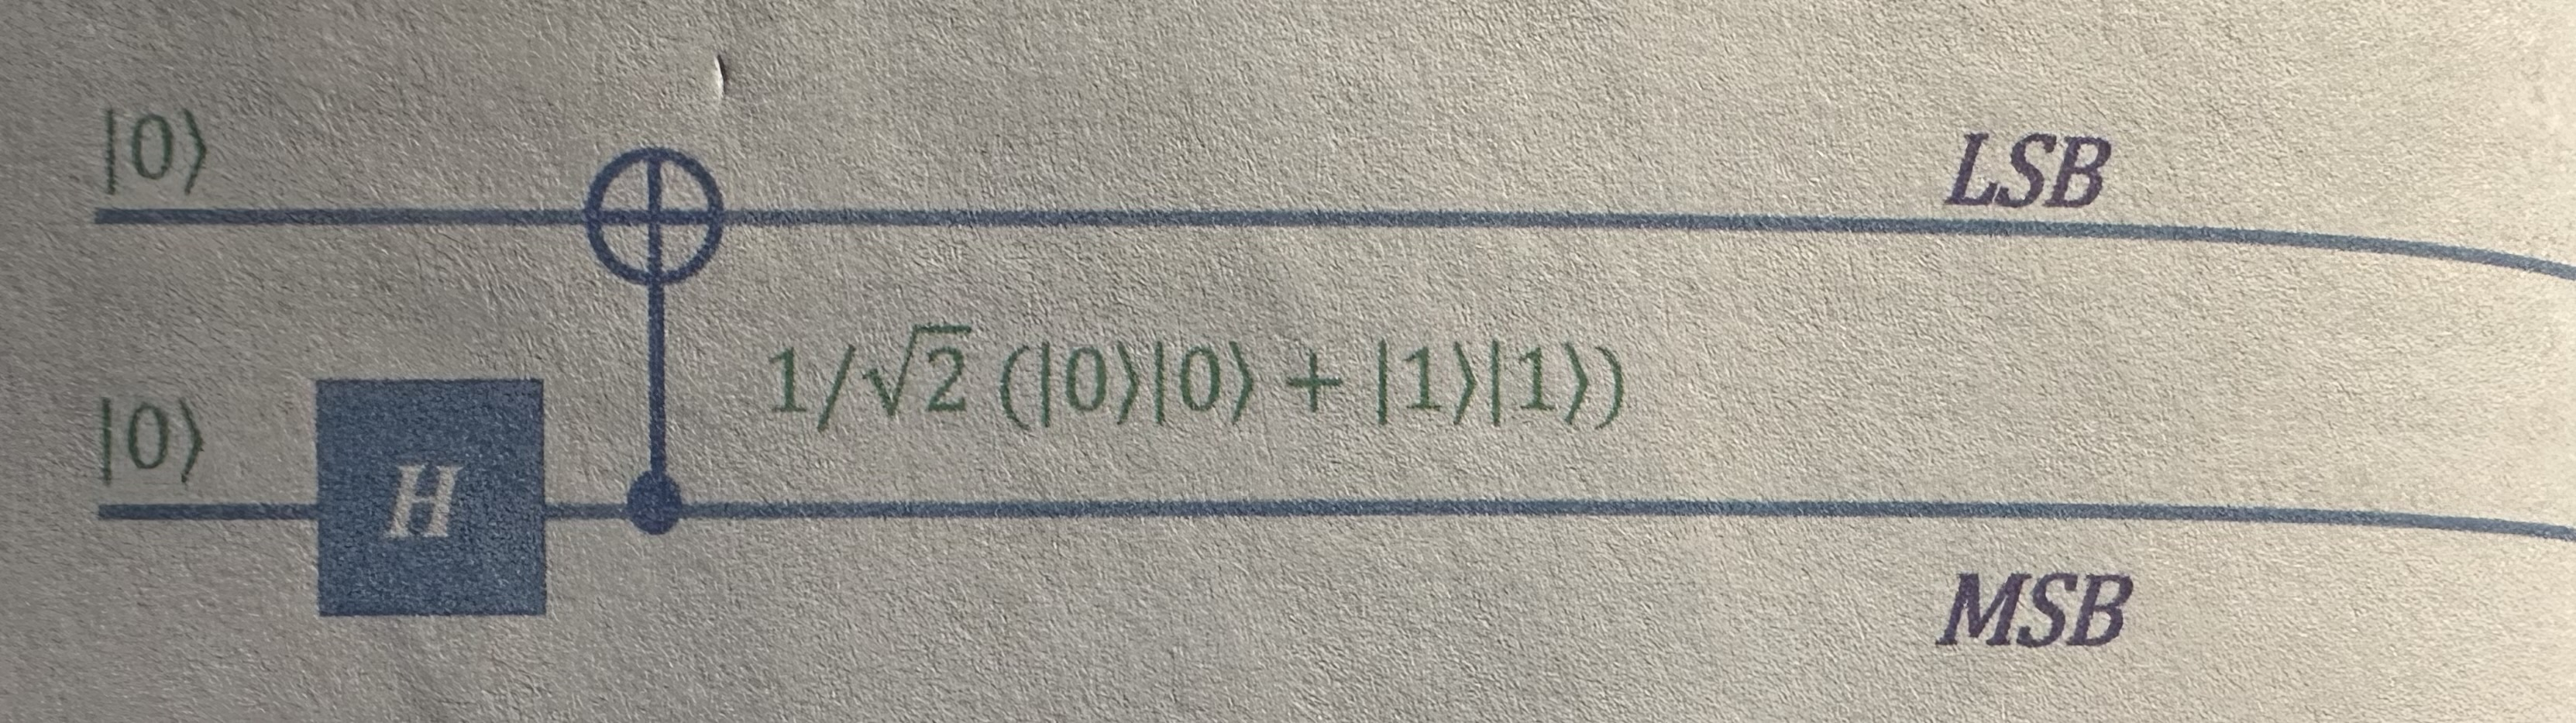
\includegraphics[scale=0.4]{Fig.12.2.jpeg}\\
\textbf{Fig.12.2} An entanglement circuit implemented  using a $\boldsymbol{U_{XOR}}$ gate and an $\boldsymbol{H}$ gate.
Note that the least significant bit (LSB) and the most significant bit (MSB) are on the top and bottom, respectively
\\\\
and the matrix form of $\boldsymbol{U_{CPS,\pi}}$ is
\begin{align*}\label{eq 12.4}
  \boldsymbol{U_{CPS,\pi}}&=\begin{pmatrix}
    1&0&0&0\\0&1&0&0\\0&0&1&0\\0&0&0&e^{i\pi}
  \end{pmatrix},\\
  &= \begin{pmatrix}
    1&0&0&0\\0&1&0&0\\0&0&1&0\\0&0&0&-1
  \end{pmatrix},\tag{12.4}
\end{align*}
as $e^{i\pi}=\cos\pi+i\sin\pi=-1$. Therefore,
\begin{align*}\label{eq 12.5}
  &(\boldsymbol{I}\otimes\boldsymbol{H})\boldsymbol{U_{CPS,\pi}}(\boldsymbol{I}\otimes\boldsymbol{H})\\[5pt]
  &=\begin{pmatrix}
    1\ 0\\ 0\ 1
  \end{pmatrix}\otimes\frac{1}{\sqrt{2}}
  \begin{pmatrix}
    1&1\\1&-1
  \end{pmatrix}\boldsymbol{U_{CPS,\pi}}
  \begin{pmatrix}
    1\ 0\\ 0\ 1
  \end{pmatrix}\otimes\frac{1}{\sqrt{2}}
  \begin{pmatrix}
    1&1\\1&-1
  \end{pmatrix},\\[5pt]
  &=\frac{1}{\sqrt{2}}\begin{pmatrix}
    1&1&0&0\\1&-1&0&0\\0&0&1&1\\0&0&1&-1
  \end{pmatrix}
  \begin{pmatrix}
    1&0&0&0\\0&1&0&0\\0&0&1&0\\0&0&0&-1
  \end{pmatrix}
  \frac{1}{\sqrt{2}}
  \begin{pmatrix}
    1&1&0&0\\1&-1&0&0\\0&0&1&1\\0&0&1&-1
  \end{pmatrix},\\[5pt]
  &=\frac{1}{2}\begin{pmatrix}
    1&1&0&0\\1&-1&0&0\\0&0&1&1\\0&0&1&-1
  \end{pmatrix}
  \begin{pmatrix}
    1&1&0&0\\1&-1&0&0\\0&0&1&1\\0&0&1&-1
  \end{pmatrix},\\[5pt]
  &=\frac{1}{2}\begin{pmatrix}
    2\ 0\ 0\ 0\\ 0\ 2\ 0\ 0\\0\ 0\ 0\ 2\\ 0\ 0\ 2\ 0
  \end{pmatrix},\\[5pt]
  &=\begin{pmatrix}
    1\ 0\ 0\ 0\\ 0\ 1\ 0\ 0\\0\ 0\ 0\ 1\\ 0\ 0\ 1\ 0
  \end{pmatrix},\\[5pt]
  &=\boldsymbol{U_{XOR}}. \tag{12.5}
\end{align*}

Now, we will show that we can implemenet $\boldsymbol{U_{CPS,\pi}}$ using $\boldsymbol{U_{Cphase}}$
and \textit{other 1-qubit gates}.
\\\\
\textbf{Example 12.2} Show that $\boldsymbol{U_{CPS,\pi}}=\boldsymbol{U_{Cphase}}(\boldsymbol{I}\otimes\boldsymbol{U_{PS,-\phi}})
(\boldsymbol{U_{PS,\phi-\pi}}\otimes\boldsymbol{I})$.

Recall that the matrix form of the pahse shift gate, $\boldsymbol{U_{PS,\phi}}$, is
\begin{equation}\label{eq 12.6}
  \begin{pmatrix}
    1&0\\0&e^{i\phi}
  \end{pmatrix}.\tag{12.6}
\end{equation}

Therefore,
\begin{equation}\label{eq 12.7}
  \boldsymbol{I}\otimes\boldsymbol{U_{PS,-\phi}}=\begin{pmatrix}
    1\ 0\\ 0\ 1
  \end{pmatrix}\otimes
  \begin{pmatrix}
    1&0\\0&e^{-i\phi}
  \end{pmatrix}=
  \begin{pmatrix}
    1&0&0&0\\0&e^{-i\phi}&0&0\\0&0&1&0\\0&0&0&e^{-i\phi}
  \end{pmatrix},\tag{12.7}
\end{equation}
and
\begin{equation}\label{eq 12.8}
  (\boldsymbol{U_{PS,\phi-\pi}}\otimes\boldsymbol{I})=
  \begin{pmatrix}
    1&0\\0&e^{i(\phi-\pi)}
  \end{pmatrix}\otimes
  \begin{pmatrix}
    1\ 0\\ 0\ 1
  \end{pmatrix}=
  \begin{pmatrix}
    1&0&0&0\\0&1&0&0\\0&0&e^{i(\phi-\pi)}&0\\0&0&0&e^{i(\phi-\pi)}
  \end{pmatrix}.\tag{12.8}
\end{equation}

Using Eqs.(\ref{eq 12.1}),(\ref{eq 12.7}), and (\ref{eq 12.8}), we have
\begin{align*}\label{eq 12.9}
 & \boldsymbol{U_{Cphase}}(\boldsymbol{I}\otimes\boldsymbol{U_{PS,-\phi}})
(\boldsymbol{U_{PS,\phi-\pi}}\otimes\boldsymbol{I})\\[5pt]
&=\begin{pmatrix}
  1&0&0&0\\0&e^{i\phi}&0&0\\0&0&e^{i(\pi-\phi)}&0\\0&0&0&1
\end{pmatrix}
\begin{pmatrix}
  1&0&0&0\\0&e^{-i\phi}&0&0\\0&0&1&0\\0&0&0&e^{-i\phi}
\end{pmatrix}
\begin{pmatrix}
  1&0&0&0\\0&1&0&0\\0&0&e^{i(\phi-\pi)}\\0&0&0&e^{i(\phi-\pi)}
\end{pmatrix},\\[5pt]
&=\begin{pmatrix}
  1&0&0&0\\0&e^{i\phi}&0&0\\0&0&e^{i(\pi-\phi)}&0\\0&0&0&1
\end{pmatrix}
\begin{pmatrix}
  1&0&0&0\\0&e^{-i\phi}&0&0\\0&0&e^{i(\phi-\pi)}&0\\0&0&0&e^{-i\pi}
\end{pmatrix},\\[5pt]
&=\begin{pmatrix}
  1&0&0&0\\0&1&0&0\\0&0&1&0\\0&0&0&e^{-i\pi}
\end{pmatrix},\\[5pt]
&=\begin{pmatrix}
  1&0&0&0\\0&1&0&0\\0&0&1&0\\0&0&0&e^{i\pi}
\end{pmatrix}=
\begin{pmatrix}
  1&0&0&0\\0&1&0&0\\0&0&1&0\\0&0&0&-1
\end{pmatrix},\\[5pt]
&=\boldsymbol{U_{CPS,\pi}},\tag{12.9}
\end{align*}

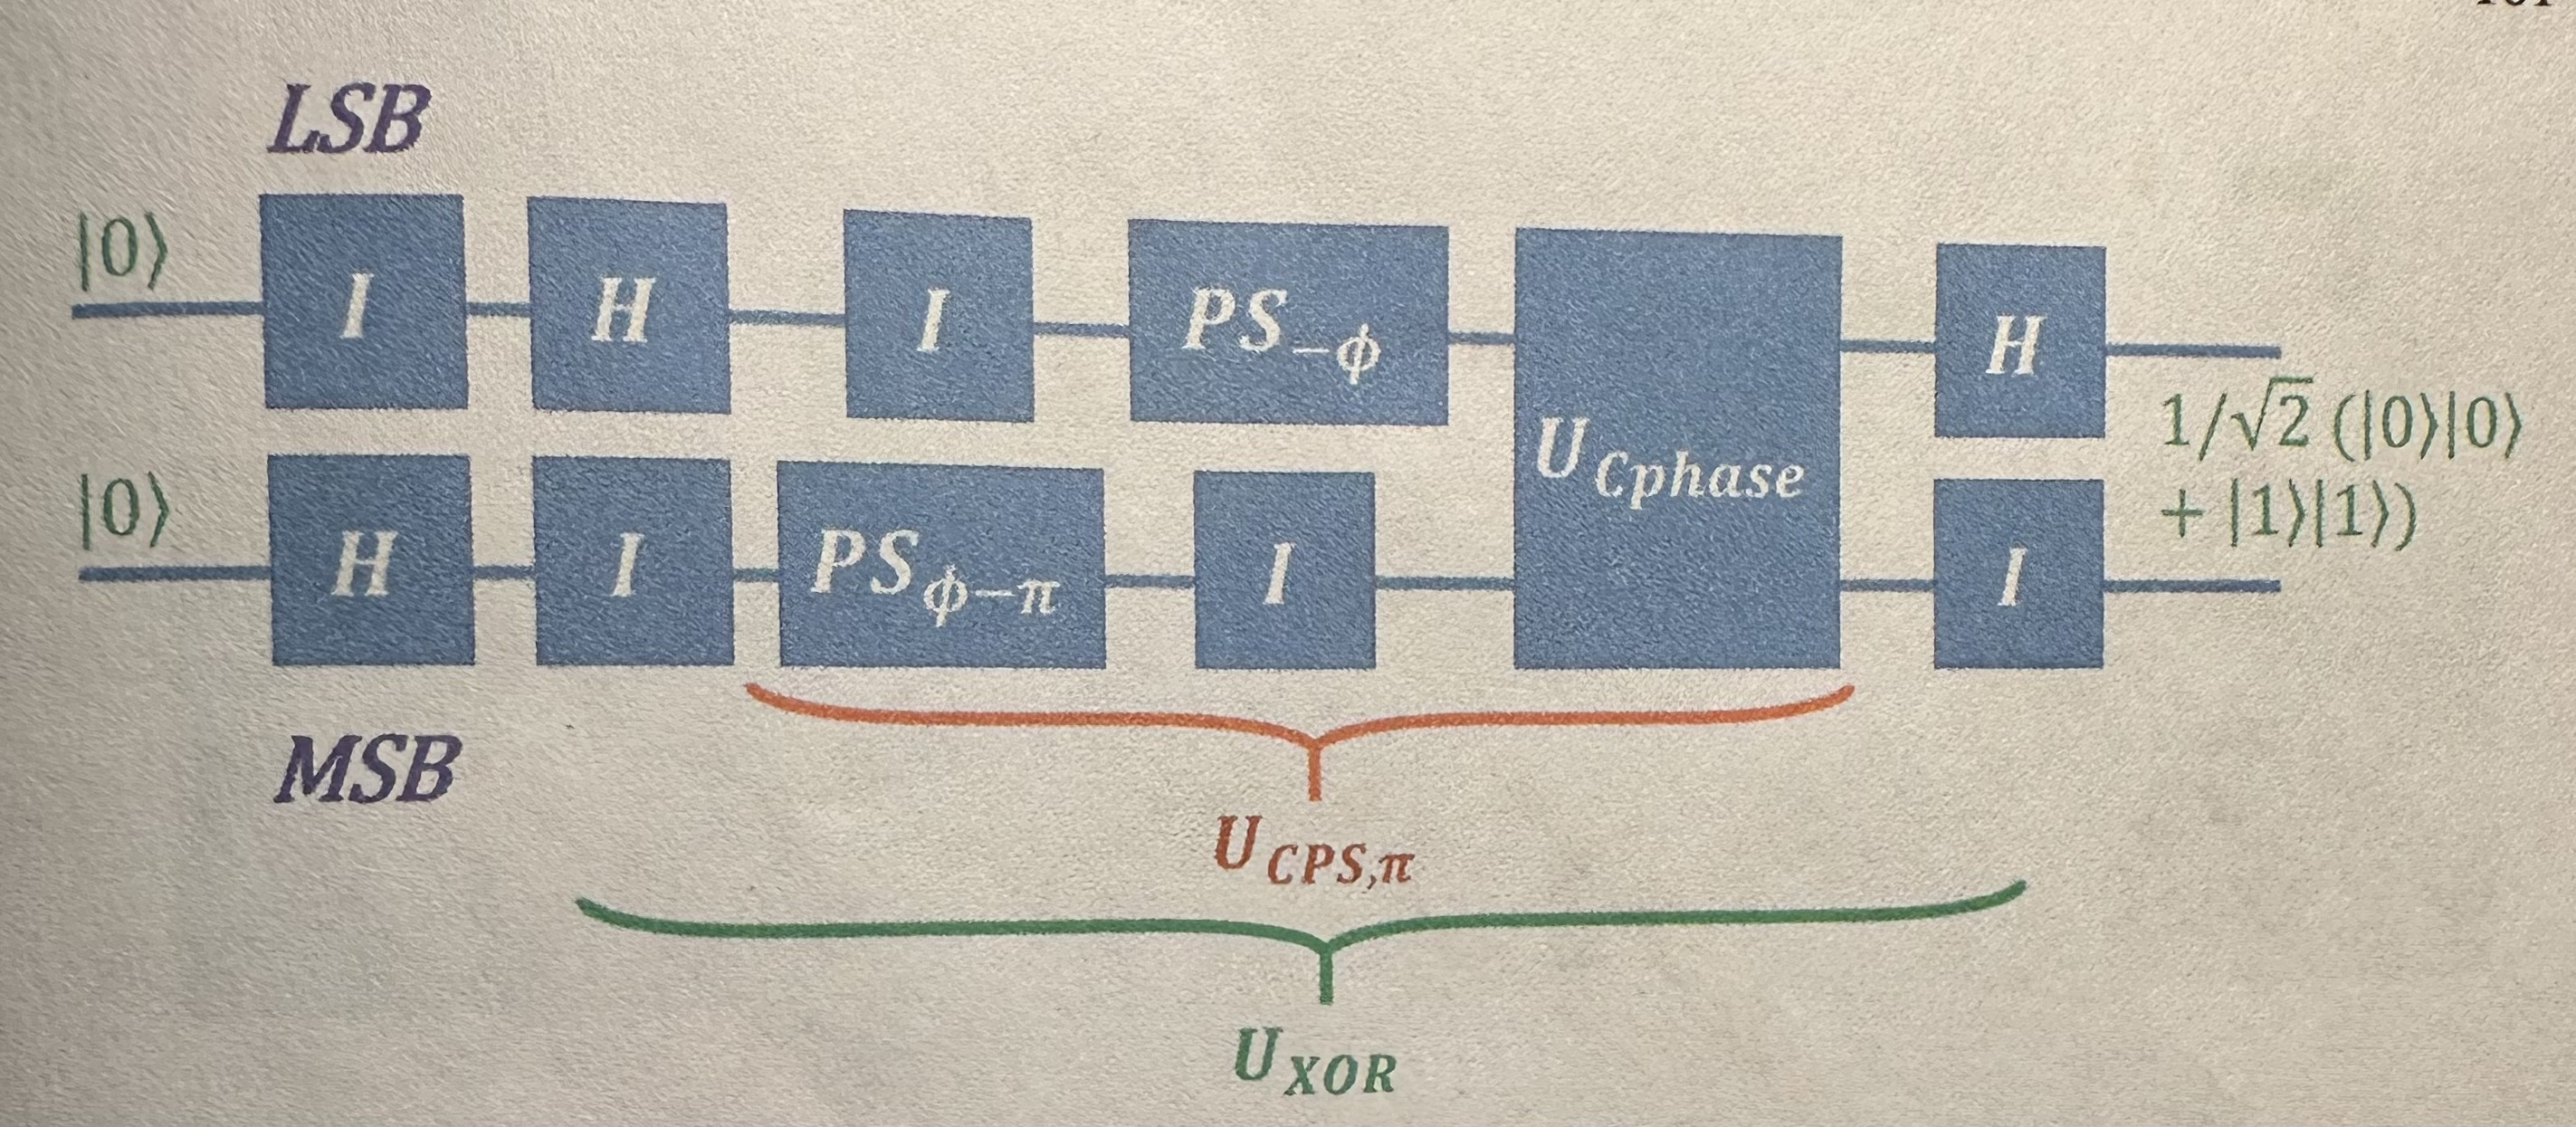
\includegraphics[scale=0.45]{Fig.12.3.jpeg}\\
\textbf{Fig.12.3} The equibalent circuit of Fig.12.2 implemented by 1-qubit gates and a $\boldsymbol{U_{Cphase}}$ gate
\\[10pt]
where at the end, we used the face that $e^{-i\pi}=e^{i\pi}$. \hfill $\blacksquare$

Therefore, we have successfully impelmented a $\boldsymbol{U_{XOR}}$ gate for entanglement Creation
using the native 2-qubit gate for electron spin. Figure 12.3 shows the full entanglement circuit using
1-qubit gates and a $\boldsymbol{U_{Cphase}}$ gate.
\\[30pt]
\bfit{\large 12.3.2 Physical Impelementation of $\boldsymbol{U_{Cphase}}$ Gate}
\\\\
\textbf{12.3.2.1 Setup and Individual 1-Qubit Operations}\\\\
We now will try to omplement the $\boldsymbol{U_{Cphase}}$ gate in Eq. (\ref{eq 12.1}). We will following
the appropriate in \cite{meunier2011efficient} and \cite{veldhorst2015two}, however, with pretty significant
modifications and simplifications. If there is only on thing that you can remember from this subsection, I hope 
you can appreciate that fact that \textit{we need to use the physics of a system to realize an entanglement gate and we need to adjust the condition so
that it can achieve the purpose most effectively}. The process of using the right physics and adjusting the conditions
is called \textbf{Hamiltonian engineering}. Again, Hamiltonian refers to the total energy of the system. So the fancy
word "Hamiltonian engineering" is nothing but setting up the system at the right energy at the right time to let it evolve
in a desirable way.

Figure 12.4 shows the schematic of two qubits on a silicon wafer. The barrier gate is not shown for
clarity. Same as the 1-qubit example in Sect. 12.2, $T=50$ mK and $B_0=1.4T$ and highly purified Si is used 
(with only 800 ppm of $^{29}Si$).

Before working on a 2-qubit gate, we need to make sure we can perform 1-qubit operation on \textit{individual} qubit.
To do so, we need to have different \textit{electron spin resonance frequency}, which is the Larmor frequency,
$\omega_L$, for each qubit. Otherwise, we will be applying the same 1-qubit gate to both qubits at the same time.
Equation (8.11) tells us that $\omega_L$ depends on $B_0$, the g-factor, $g$, and the effective mass of the electron, 
$m^*$, which is repeated here for convenience.\\[6pt]

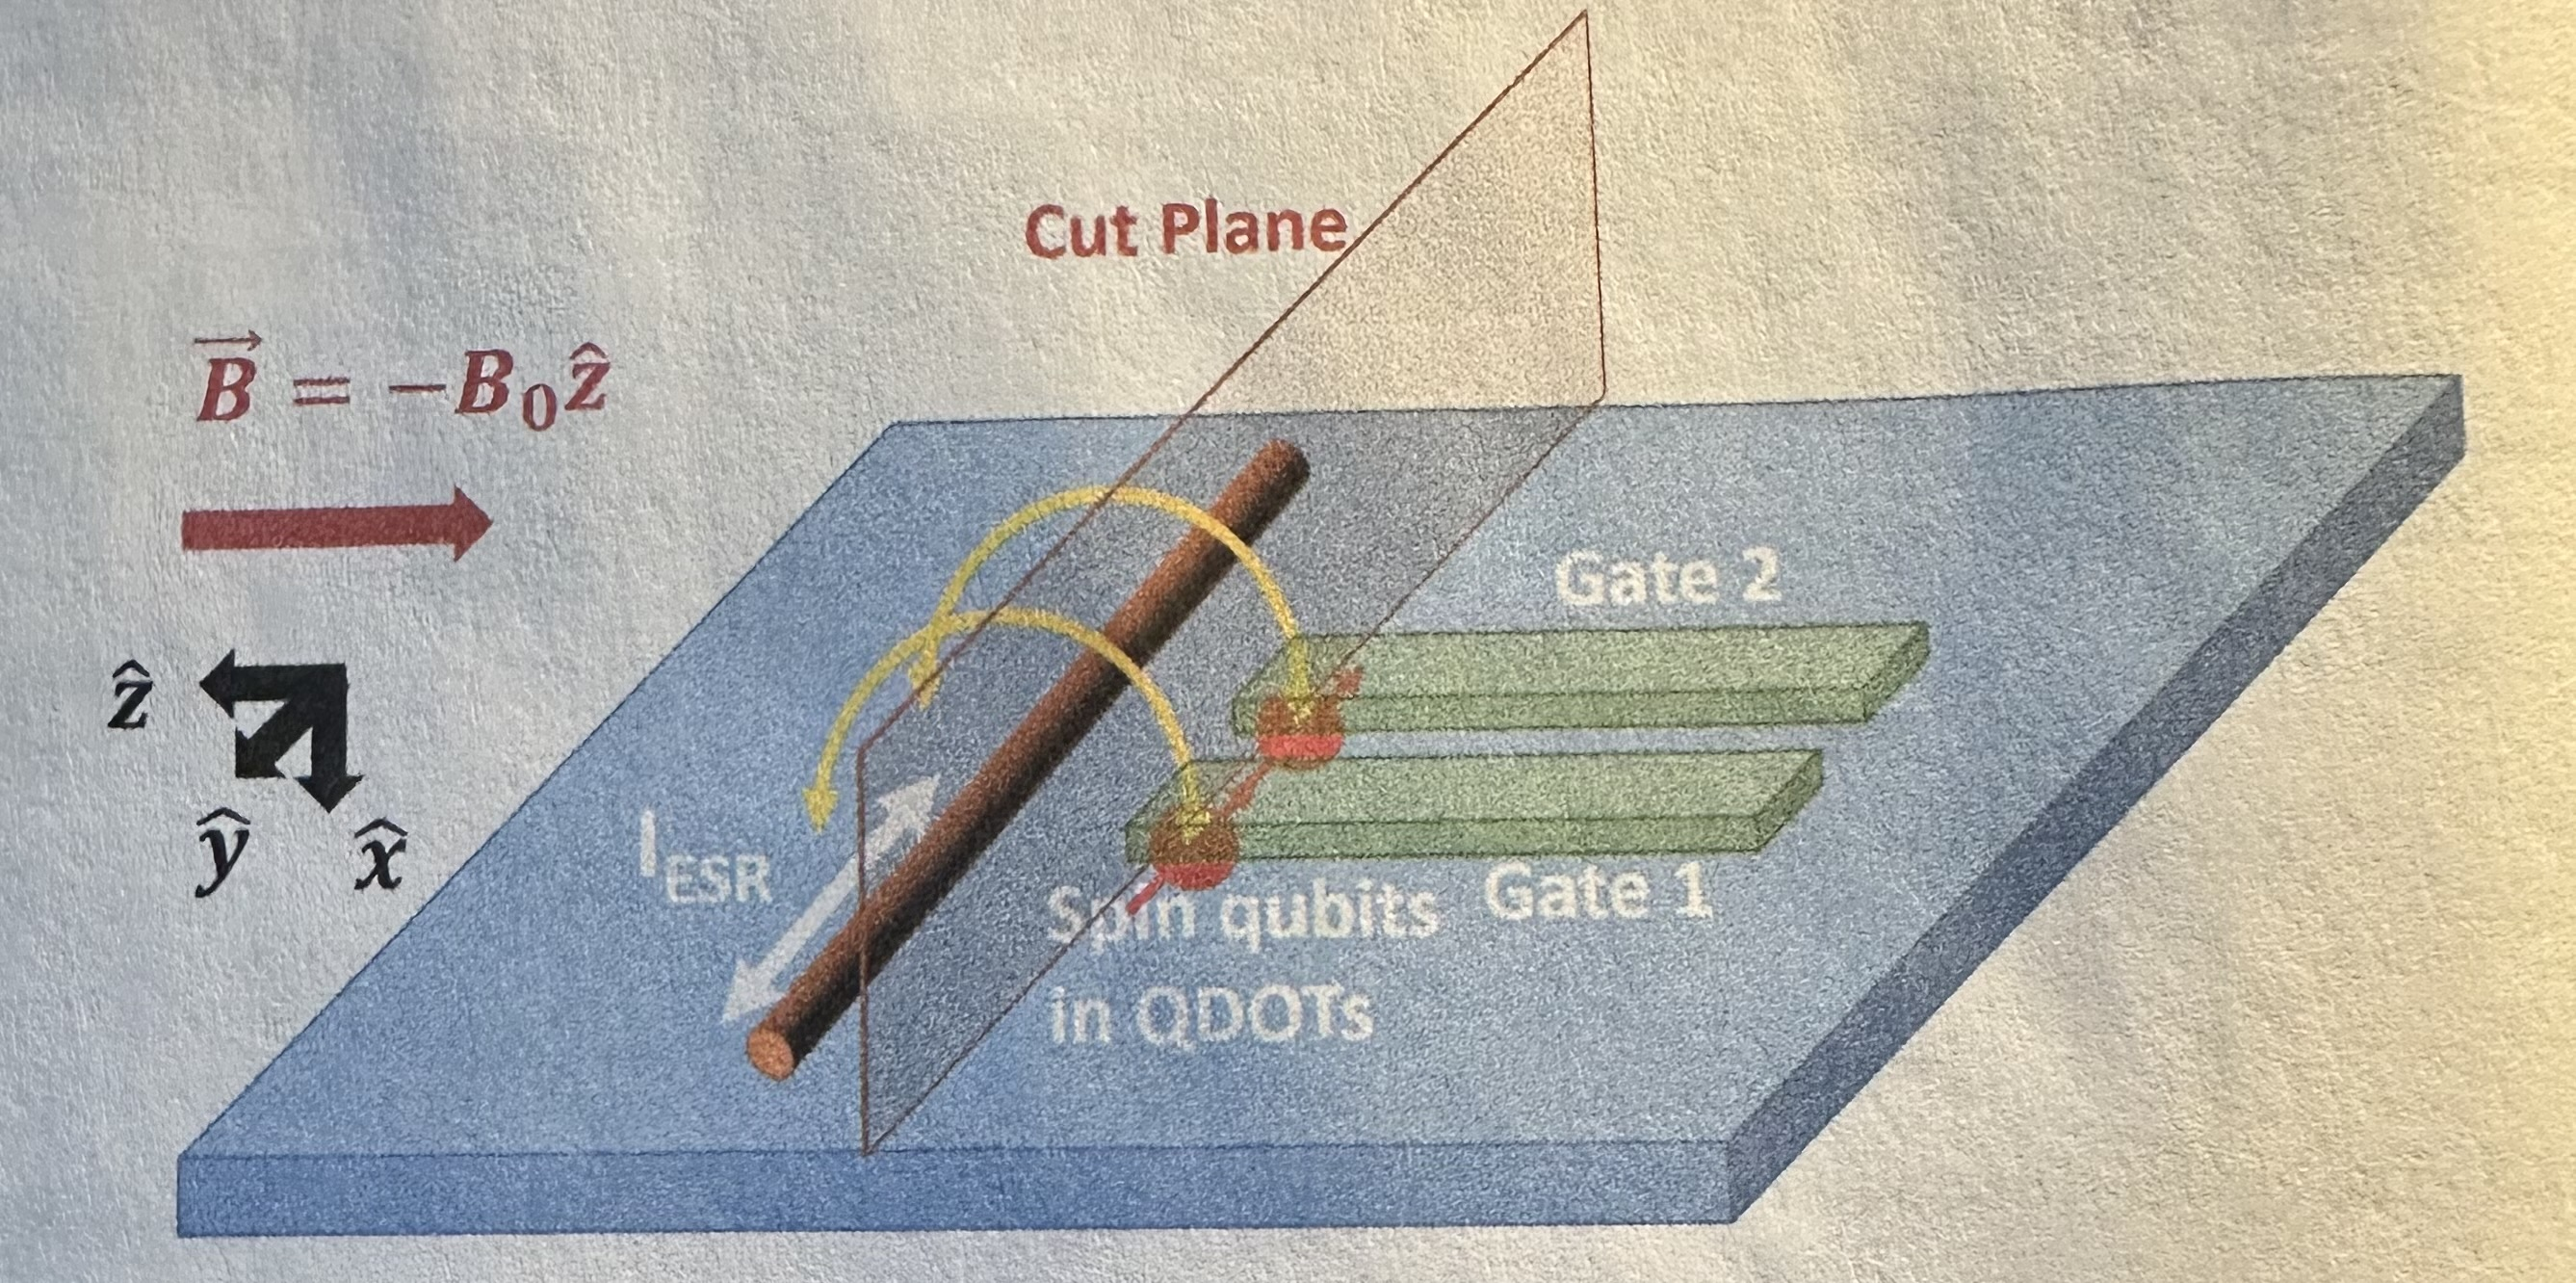
\includegraphics[scale=0.45]{Fig.12.4.jpeg}
\\
\textbf{Fig.12.4} Schematic showing a 2-qubit system. The barrier gate is not used
\\[10pt]
\begin{equation}\label{eq 12.10}
  \omega_L=\left|\frac{2ge\hbar}{4m^*}B_o\right|/\hbar. \tag{12.10}
\end{equation}

$B_0$ can be set to be different at each qubit by putting a micro-magent with a diffetent
strength nex to each qubit. However, this is not very scalable when millions of qubits need to
be integrated. Instead of using micro-magnet, with some engineering, it is also possible to create
a non-constant DC magnetic field (but still constant and pointing in $-\hat{z}$ direction) from
qubit to qubit. $m^*$ is likely to be the sam ebecause the crystal properties would not change
much across the chip. Another approach is to change $g$ which can be affected by the electric field
it experiences through \textbf{Stark effect} \cite{veldhorst2014addressable}. This is very convenient 
because it means that we can just apply different plunger gate boltages (in combination with other electrodes)
to achieve different plunger gate voltages (in combination with other electrodes) to achieve different
$\omega_L$ for each qubit. We can then change the frequency of $I_{ESR}$ so that we can address individual qubits.
This is called \textbf{spectral selectivity} as we are selecting qubits based on frequency.

For example, qubit 1 might have $\omega_L=0.34MHz$ and qubit 1 might have $\omega_L=0.36MHz$.
By setting $I_{ESR}$ to oscillate at $0.34MHz$, only qubit 1 will perform Rabi oscillation as it
is at its spin resonance. Qubit 2 wil not as it is off-resonant.\\[15pt]
\textbf{12.3.2.2 2-Qubit Physics}\\\\
The physics and the mathematics of implementing the 2-qubit $\boldsymbol{U_{Cphase}}$ gate is pretty 
complicated and lenghty. We will not go thorough all the derivation here. We will only highlight the critical concpets so we 
can appreciate what the enabler is.

Figure 12.5 shows the corss section of the 2-qubit array. The gates are biased at different voltages.
As a result, they have different $\omega_L$ as discussed earlier due to \textit{Stark effect}.\\[5pt]

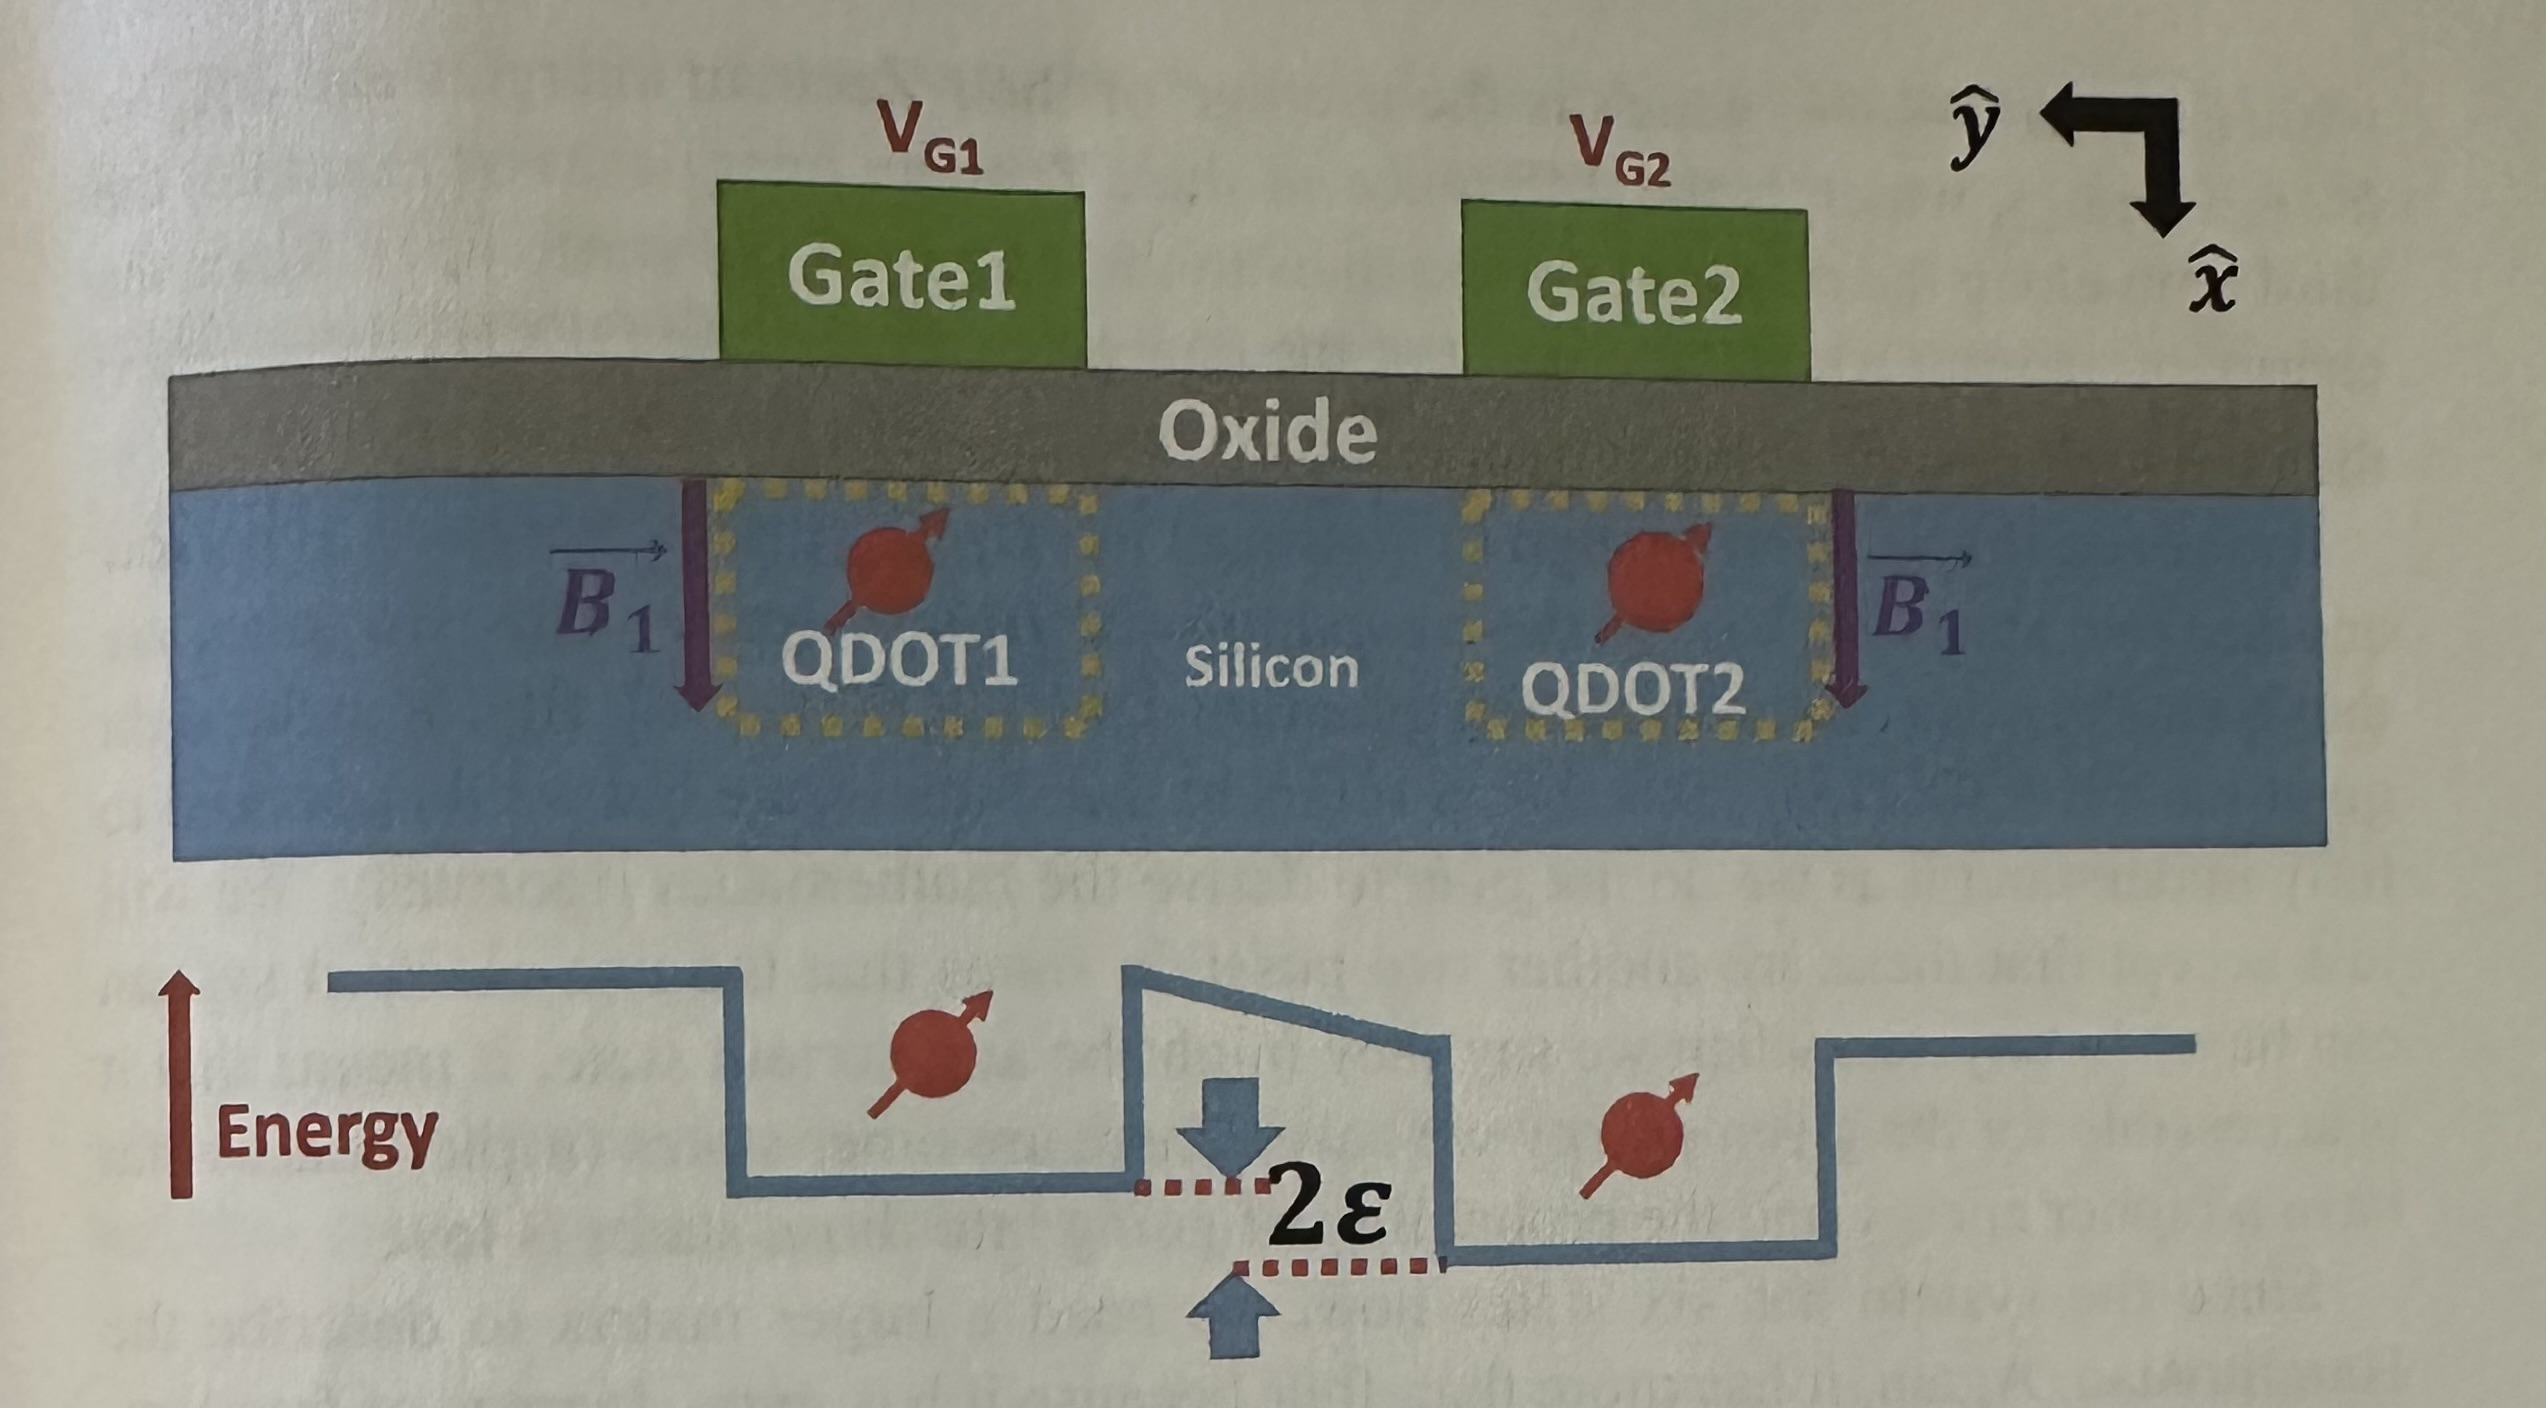
\includegraphics[scale=0.5]{Fig.12.5.jpeg}\\
\textbf{Fig. 12.5} Cut plane in Fig. 12.4 and the corresponding electron potential energy along the quantum dot.
$V_{G2}$ is more positive than $V_{G1}$\\[5pt]

Since this is a 2-qubit system. it has four basis states. One of the choices of the basis state
is $\ket{\uparrow\uparrow},\ket{\uparrow\downarrow},\ket{\downarrow\uparrow},$ and $\ket{\downarrow\downarrow}$.
When we write them in $bra-ket$ notation, the first one refers to the electron in the left quantum
dot and the second on refers to the electron in the right quantum dot. For each qubit, according to Eqs.(8.4) and (8.11),
its Hamiltonian is,
\begin{align*}\label{eq 12.11}
  \boldsymbol{H_i}&=B_0\frac{\text{g}e\hbar}{4m}\begin{pmatrix}
    1& 0\\ 0& -1
  \end{pmatrix},\\
  &=-\frac{\hbar\omega_{Li}}{2}\begin{pmatrix}
    1&0\\0&-1
  \end{pmatrix}\\
  &= \begin{pmatrix}
    -\frac{\hbar\omega_{Li}}{2}&0\\0&\frac{\hbar\omega_{Li}}{2}
  \end{pmatrix},\tag{12.11}
\end{align*}
where $i=1$ and $i=2$ for the qubit in QDOT1 and QDOT2, respectively.

Therefore, the Hamiltonian of the system, which can be obtained by the tensor product
of the individual Hamiltonian, is
\begin{equation}\label{eq 12.12}
  \boldsymbol{H}=\begin{pmatrix}
    -E_z&0&0&0\\0&\frac{-dE_z}{2}&0&0\\0&0&\frac{dE_z}{2}&0\\0&0&0&E_z
  \end{pmatrix},\tag{12.12}
\end{equation}
with $E_z=\hbar\frac{\omega_{L1}+\omega_{L2}}{2}$, which is the average of their Zeeman energies and
$dE_z=\hbar\omega_{L1}-\hbar\omega_{L2}$, which is the difference of their Zeeman energies. For example, 
the third term along the diagoanl corresponds to the energy of the state, $\ket{\uparrow\downarrow}$. Since
the energy of $\ket{\downarrow}$ in QDOT1 is $\frac{\hbar\omega_{L1}}{2}$ and the energy of $\ket{\uparrow}$
in the QDOT2 is $-\frac{\hbar\omega_{L2}}{2}$, then the total energy of the system is $\frac{\hbar\omega_{L1}}{2}-\frac{\hbar\omega_{L2}}{2}=\frac{dE_z}{2}$.

However, this is $NOT$ enough to construct the $\boldsymbol{U_{Cphase}}$ gate. We need to borrow another two states 
\textit{outside of the computational Hiblert space}. The two states are that both electrons
can be in the quantum dot (QDOT1), $\ket{S(2,0)}$, or in the right quantum dot
(QDOT2), $\ket{S(0,2)}$. $S$ refers to the singlet state but we do not need to fully
understand it as we do not plan to derive the mathematics rigorously. We will just
accept that these are another two possible states that the two-electron system can have.
In physics, when we say they might be at a certain state, it means that it is accessible
for the given energy we have. There are other states (triple states) that have a higher energy
and the probability of going into those states is low.

Since the system has six states now, we need a larger matrix to describe the Hamiltonian.
Again, it has more than four because it has extra degrees of freedon, namely, where to put
the electrons. The Hamiltonian is,
\begin{equation}\label{eq 12.13}
  \boldsymbol{H}=\begin{pmatrix}
    -E_z&0&0&0&0&0\\[3pt]0&\frac{-dE_z}{2}&0&0&t&t\\[3pt]0&0&\frac{dE_z}{2}&0&-t&-t\\[3pt]
    0&0&0&E_z&0&0\\[3pt]0&t&-t&0&U-\epsilon&0\\[3pt]0&t&-t&0&0&U+\epsilon
  \end{pmatrix}
  \begin{matrix}
    \ket{\uparrow\uparrow}\\[3pt]
    \ket{\uparrow\downarrow}\\[3pt]
    \ket{\downarrow\uparrow}\\[3pt]
    \ket{\downarrow\downarrow}\\[3pt]
    S(0,2)\\[3pt]
    S(2,0)
  \end{matrix},\tag{12.13}
\end{equation}
where $U$ is the energy cost to move the two electrons to the same quantum dot (see the
\textbf{charging energy} and \textbf{Coulomb blockade} discussed in Sect. 11.3) and $\epsilon$
is the energy difference between the two dots as shown in Fig.12.5. The fifth and the sixth
term along the diagonal are the energy of $\ket{S(0,2)}$ and $\ket{(2,0)}$. For example, to put
both electrons in QDOT2 ($\ket{S(0,2)}$), we need an energy of $U$. However, it has a lower energy 
due to the tilted potential by $\epsilon$. Therefore, its energy is $U-\epsilon$.

The state associated with each row is also given. We see that there are off-diagoanl terms connecting the
anti-parallel spin states ($\ket{\uparrow\downarrow}$ and $\ket{\downarrow\uparrow}$ to $\ket{S(0,2)}$
and $\ket{S(2,0)})$. This is due to \textbf{tunneling} and the value $t$ is related to the tunneling rate.
This is easy to understand as to have a state with both electrons in QDOT1 or QDOT2, tunneling through the 
barrier is required. Therefore, $t$ is called the interdot tunnel coupling. Tunneling enables the two qubits to 
interact and the tunneling rate is contolled by the barrier height between the two quantum dots through
the barrier gate voltage (not drawn in Fig. 12.5). But why there is no coupling between
the parallel spin states ($\ket{\uparrow\uparrow}$ and $\ket{\downarrow\downarrow}$) to $\ket{S(0,2)}$
and $\ket{S(2,0)}$? This is because $\ket{S(0,2)}$ and $\ket{S(2,0)}$ are singlet states in which the spins are 
anti-parallel. Therefore, parallel spin states of $\ket{\uparrow\uparrow}$ and $\ket{\downarrow\downarrow}$ cannot
transit to $\ket{S(0,2)}$ and $\ket{S(2,0)}$ easily as spin flipping is needed.

Now, if we chagne $\epsilon$ fro zero, the energies of the anti=parallel states will change
due to the coupling to $\ket{S(0,2)}$ and $\ket{S(2,0)}$. However, the energies of the parallel
states will NOT change as they are not coupled to $\ket{S(0,2)}$ and $\ket{S(2,0)}$. Therefore,
\textbf{additional phase shift will be added to the anti-parallel spin states}, $\ket{\uparrow\downarrow}$ \textbf{and}
$\ket{\downarrow\uparrow}$ but not the paralle state after solving the Schr\"{o}dinger equation (using the Schrieffer
-Wolff transformation) and the gate has the following form:
\begin{equation}\label{eq 12.14}
  \begin{pmatrix}
    1&0&0&0\\0&e^{i\phi_1}&0&0\\0&0&e^{i\phi_2}&0\\0&0&0&1
  \end{pmatrix}.\tag{12.14}
\end{equation}
where $\phi_1$ and $\phi_2$ are phases. By applying large enough $dE_z$, we can set $\phi_1=
\pi-\phi_2$ and thus create the $\boldsymbol{U_{Cphase}}$ gate in Eq.(\ref{eq 12.1}).
\\[20pt]
\textbf{\large 12.4 Summary}
\\\\
In this chapter, we have discussed how to implement Rabi oscillation on electron spin qubits integrated on a silicon chip.
An external DC magnetic field (can be due to micro-magnet) is applied for Zeeman splitting. A wire conducting
AC electric current is used to generate an AC perturbation field for Rabi oscillation. We also discuss
how to implement a 2-qubit entanglement gate ($\boldsymbol{U_{Cphase}}$) through the coupling of the anti-parallel
spin state to $\ket{S(0,2)}$ and $\ket{S(2,0)}$. $\boldsymbol{U_{Cphase}}$ is just one of the possible
entanglement gates but it highlights the importance of Hamiltonian engineering.
\\[20pt]
\textbf{\large Problems}
\\\\
\textbf{12.1 2-Qubit Hamiltonian}\\
Derivce Eq.(\ref{eq 12.12}) using the tensor product of $\boldsymbol{H_1}$ and $\boldsymbol{H_2}$.
\\\\
\textbf{12.2 Oscillating MAgnetic Field Generation}
\\
What is the peak current required to create 0.01T of peak oscillating magnetic field
if the conducting wire is 1$\mu m$ away from the qubit? Assume an effective dielectric constant
of 6.1. You may use Eq. (24.17).

\printbibliography
\end{document}
